\documentclass{article}
\usepackage[table,xcdraw]{xcolor}
\usepackage[spanish,es-noquoting]{babel}
\usepackage[utf8]{inputenc}
\usepackage{float}
\usepackage{todonotes}
\usepackage{subfigure}
\usepackage{hhline}
\usepackage{fancyhdr}
\pagestyle{fancy}
\fancyhf{}
\rhead{SOMA - Optomecánica abierta}
\lhead{Rueda de Filtros de diseño abierto}
\rfoot{Página \thepage}

%\usepackage[T1]{fontenc}


\graphicspath{{./img/}}
\renewcommand{\headrulewidth}{0pt}
\renewcommand{\familydefault}{\sfdefault}
%\marginsize{3cm}{3cm}{3cm}{3cm}

\title{Optomecánica abierta}
\begin{document}


\hfill \textbf{http://lec.df.uba.ar/soma}
\noindent
\rule{\linewidth}{0.5mm} \\[0.3cm]
{ \Large \bfseries Rueda de Filtros FW10 \\[0.3cm] }
\rule{\linewidth}{0.5mm}


\begin{figure}[H]
\centering
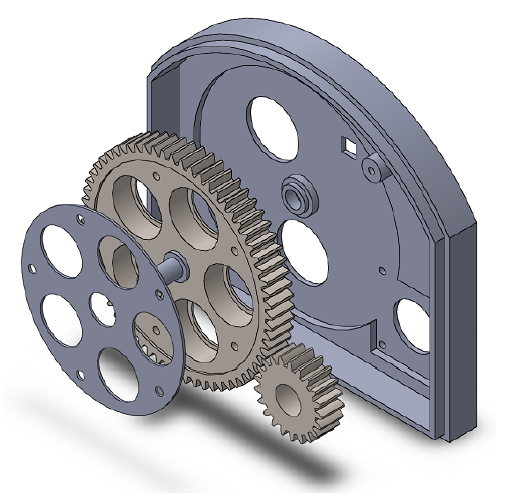
\includegraphics[width = 10cm]{ensamble1.png}
\caption{Vista isométrica de la rueda de filtros}
\label{fig:cny70:circuito}
\end{figure}

\section*{Características}
\begin{itemize}
\item Tiempo de intercambio menor a 0,2s
\item Diseño abierto y reproducible
\item 5 posiciones para filtros de 1” y hasta 7mm de espesor
\item secuencias de filtros programables

\end{itemize}

\section*{Descripción}
La rueda de filtros del sistema de optomecánica abierta consiste en un sistema de engranajes, confeccionados mediante una impresora 3D, con asientos para 5 filtros de 1” y hasta 7 mm de espesor. Un motor por pasos mueve la rueda y un sensor de proximidad permite ubicar el filtro seleccionado. El sistema se enmarca en una carcasa plástica impresa en 3D que minimiza el ruido producido por el paso de luz externa.\\

\section*{Especificaciones técnicas}

La rueda de filtros contiene un juego de engranajes de modulo 1.5 y ángulo de presión de 20º. El engranaje tiene 63 dientes con un buje central y 5 asientos para filtros de 1” y hasta 7mm de espesor. Dicho engranaje tiene 11.5mm de espesor. Por otro lado, el piñón tiene 23 dientes, mismo espesor y un orificio central que permite adherirlo al eje del motor. Ambos engranajes pueden confeccionarse mediante impresión 3D, incluso con baja calidad RepRap, y por lo tanto puede modificarse para cumplir con distintos requisitos. Los bujes y ejes fueron manufacturados en bronce. En la siguiente tabla se especifican algunas de las características actuales.

\begin{table}[H]
\centering
\parbox{.45\linewidth}{
\begin{tabular}{|l|l|}
\hline
\multicolumn{2}{ |c|} {Rueda de Filtros}  \\ \hline
Modulo     & 1.5     \\ \cline{1-2}
Ángulo de presión     & 20º     \\ \cline{1-2}
Material  & PLA \\ \cline{1-2}
Cantidad de dientes   & 63     \\ \hline
\multicolumn{2}{|c|}{Especificaciones para filtros}  \\ \cline{1-2}
Diámetro del filtro		&   1" (25,4mm)      \\ \cline{1-2}
Espesor máximo		&   7mm      \\ \cline{1-2}
Cantidad de filtros		&   5     \\ \cline{1-2}
\end{tabular}
}
\hfill
\parbox{.45\linewidth}{
\begin{tabular}{|l|l|}
\hline
\multicolumn{2}{ |c|} {Piñón}  \\ \hline
Modulo     & 1.5     \\ \cline{1-2}
Ángulo de presión     & 20º     \\ \cline{1-2}
Material  & PLA \\ \cline{1-2}
Cantidad de dientes   & 23     \\ \hline
\end{tabular}
}
\end{table}

Con el objetivo de identificar la posición de la rueda de filtros se adjuntó al sistema un optosensor por reflexión CNY-70. Se utiliza un material reflectante adherido a la rueda de filtros para marcar una posición preferencial. Agregando al optosensor los componentes electrónicos de la figura \ref{fig:cny70:circuito} y a partir de la caída de tensión en la resistencia (100K$\Omega$) se puede apreciar cuando la rueda pasa por la posición marcada.

\begin{figure}[H]
\centering
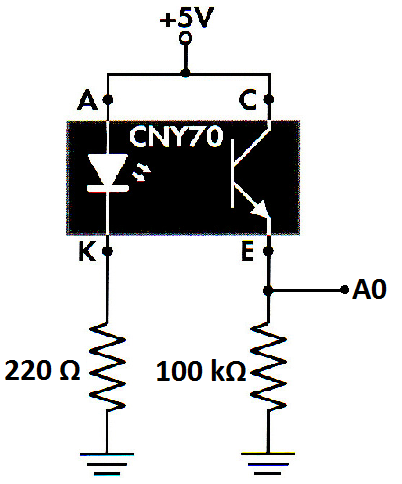
\includegraphics[height = 5cm]{CNY70-circuit.png}
\caption{Componentes electrónicos del optosensor por reflexión}
\label{fig:cny70:circuito}
\end{figure}

\begin{table}[H]
\centering
\parbox{.45\linewidth}{
\begin{tabular}{|l|l|}
\hline
\multicolumn{2}{ |c|} {Optosensor}  \\ \hline
Voltaje     & 5V     \\ \cline{1-2}
Corriente     & 25mA     \\ \cline{1-2}
Material Reflectante  & papel aluminio \\ \cline{1-2}
Voltaje umbral   & 4.5V (para aluminio)    \\ \hline
\multicolumn{2}{|c|}{Resistencias utilizadas}  \\ \cline{1-2}
Fotodiodo		&   220$\Omega$      \\ \cline{1-2}
Fototransistor		&   100k$\Omega$      \\ \cline{1-2}
Cantidad de filtros		&   5     \\ \cline{1-2}
\end{tabular}
}
\end{table}


La carcasa de la rueda de filtros no sólo sirve para minimizar el ruido producido por el paso de luz externa, sino que también provee de sostén al motor, bujes y optosensor. Una de las mitades de la carcasa sostiene el sistema, mientras que la otra complementa de manera tal de aislarla de luz externa, dando la posibilidad de probar el sistema con la carcasa abierta. La carcasa entera puede ser confeccionada mediante impresión 3D, con baja calidad, teniendo un tamaño máximo de 130x150x25mm$^3$.


\section*{Aplicaciones típicas}

La rueda de filtros fue originalmente diseñada para automatizar la captura de imágenes en procesos dinámicos con microscopía de fluorescencia. Dado que las piezas son confeccionadas mediante impresora 3D, lo que facilita su fabricación y reposición, brinda versatilidad en la adaptación de los dispositivos para su aplicación en diferentes sistema ópticos. Puede utilizarse para seleccionar filtros de forma remota, como para generar una secuencia de intercambio de filtros intercalada con captura de imágenes.

\section*{Diagramas y planos}
\begin{figure}[ht]
\centering
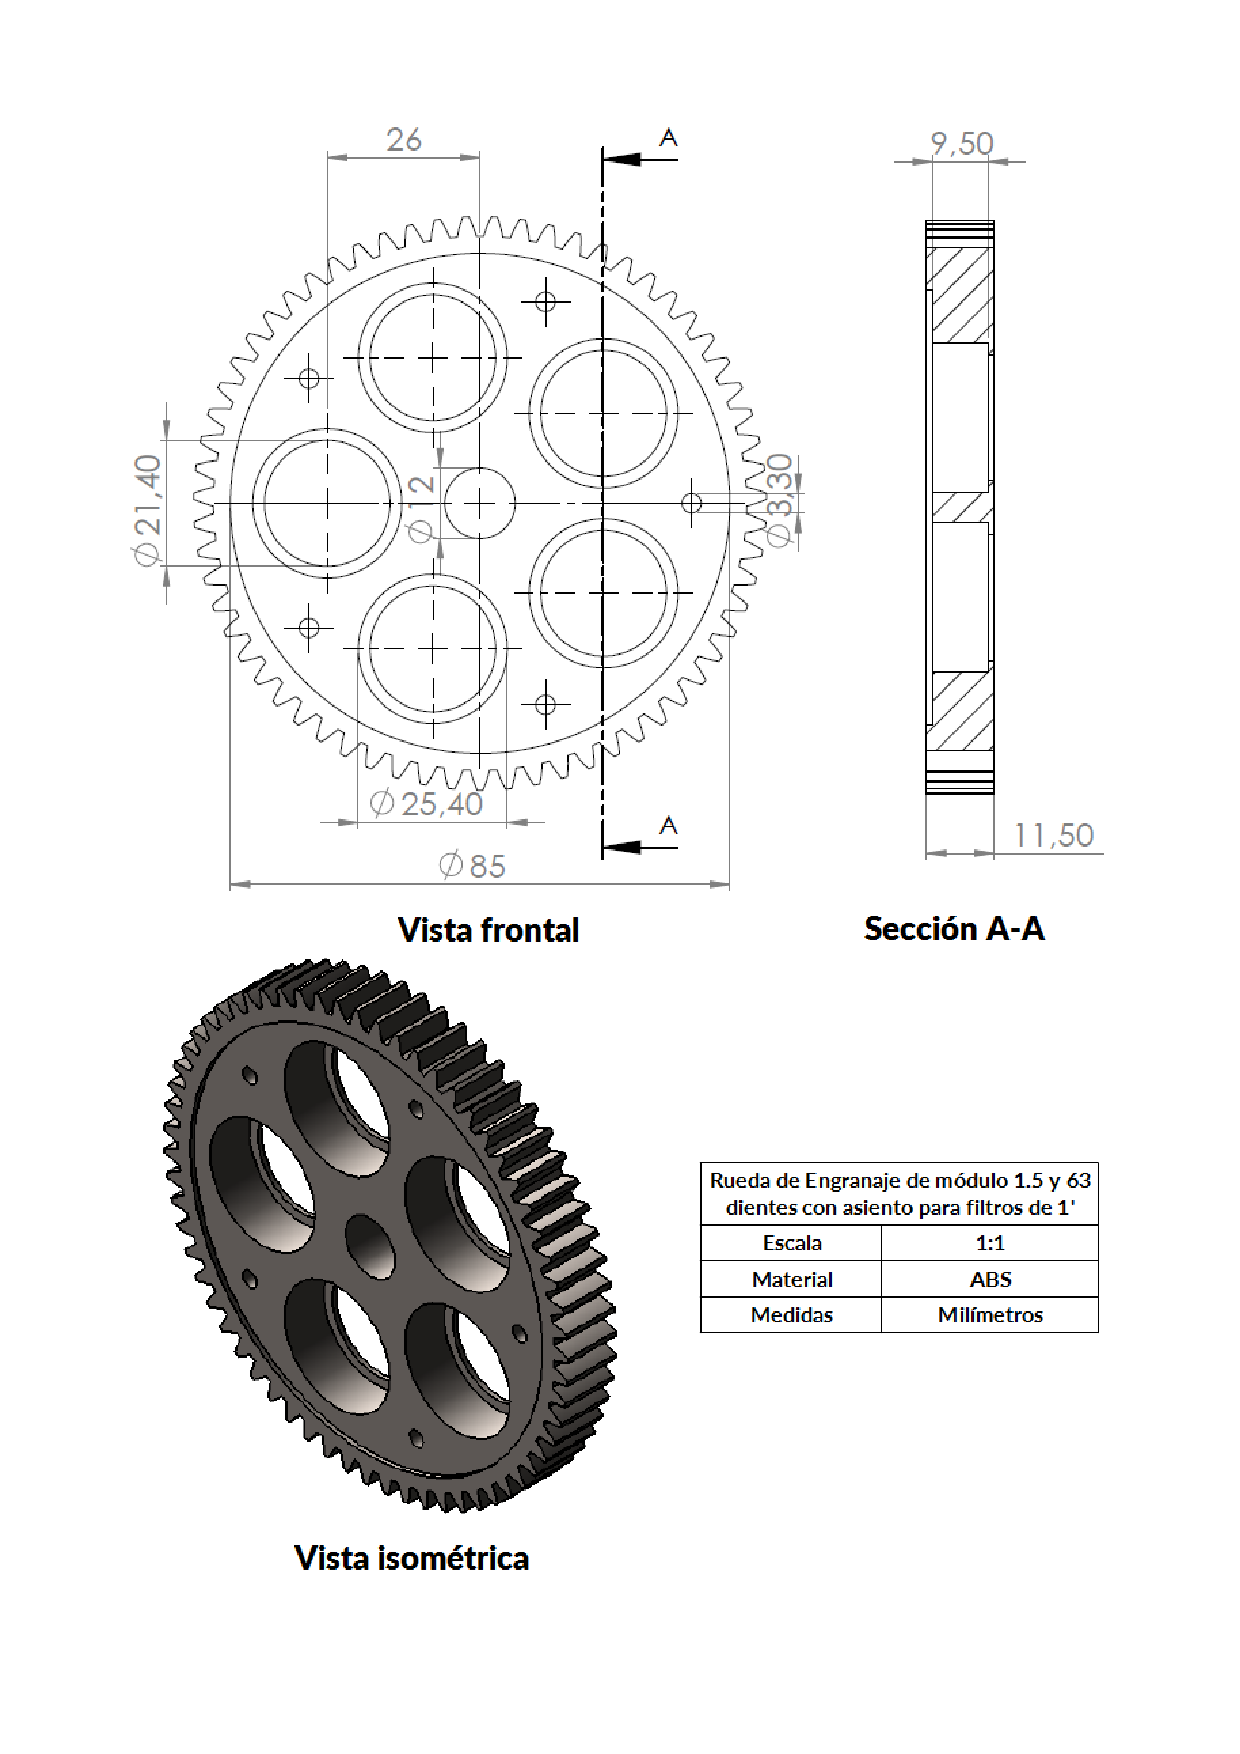
\includegraphics[height=0.72\textheight]{PlanoRueda.pdf}
\caption{Rueda de Filtros.}
\end{figure}

\begin{figure}[ht]
\centering
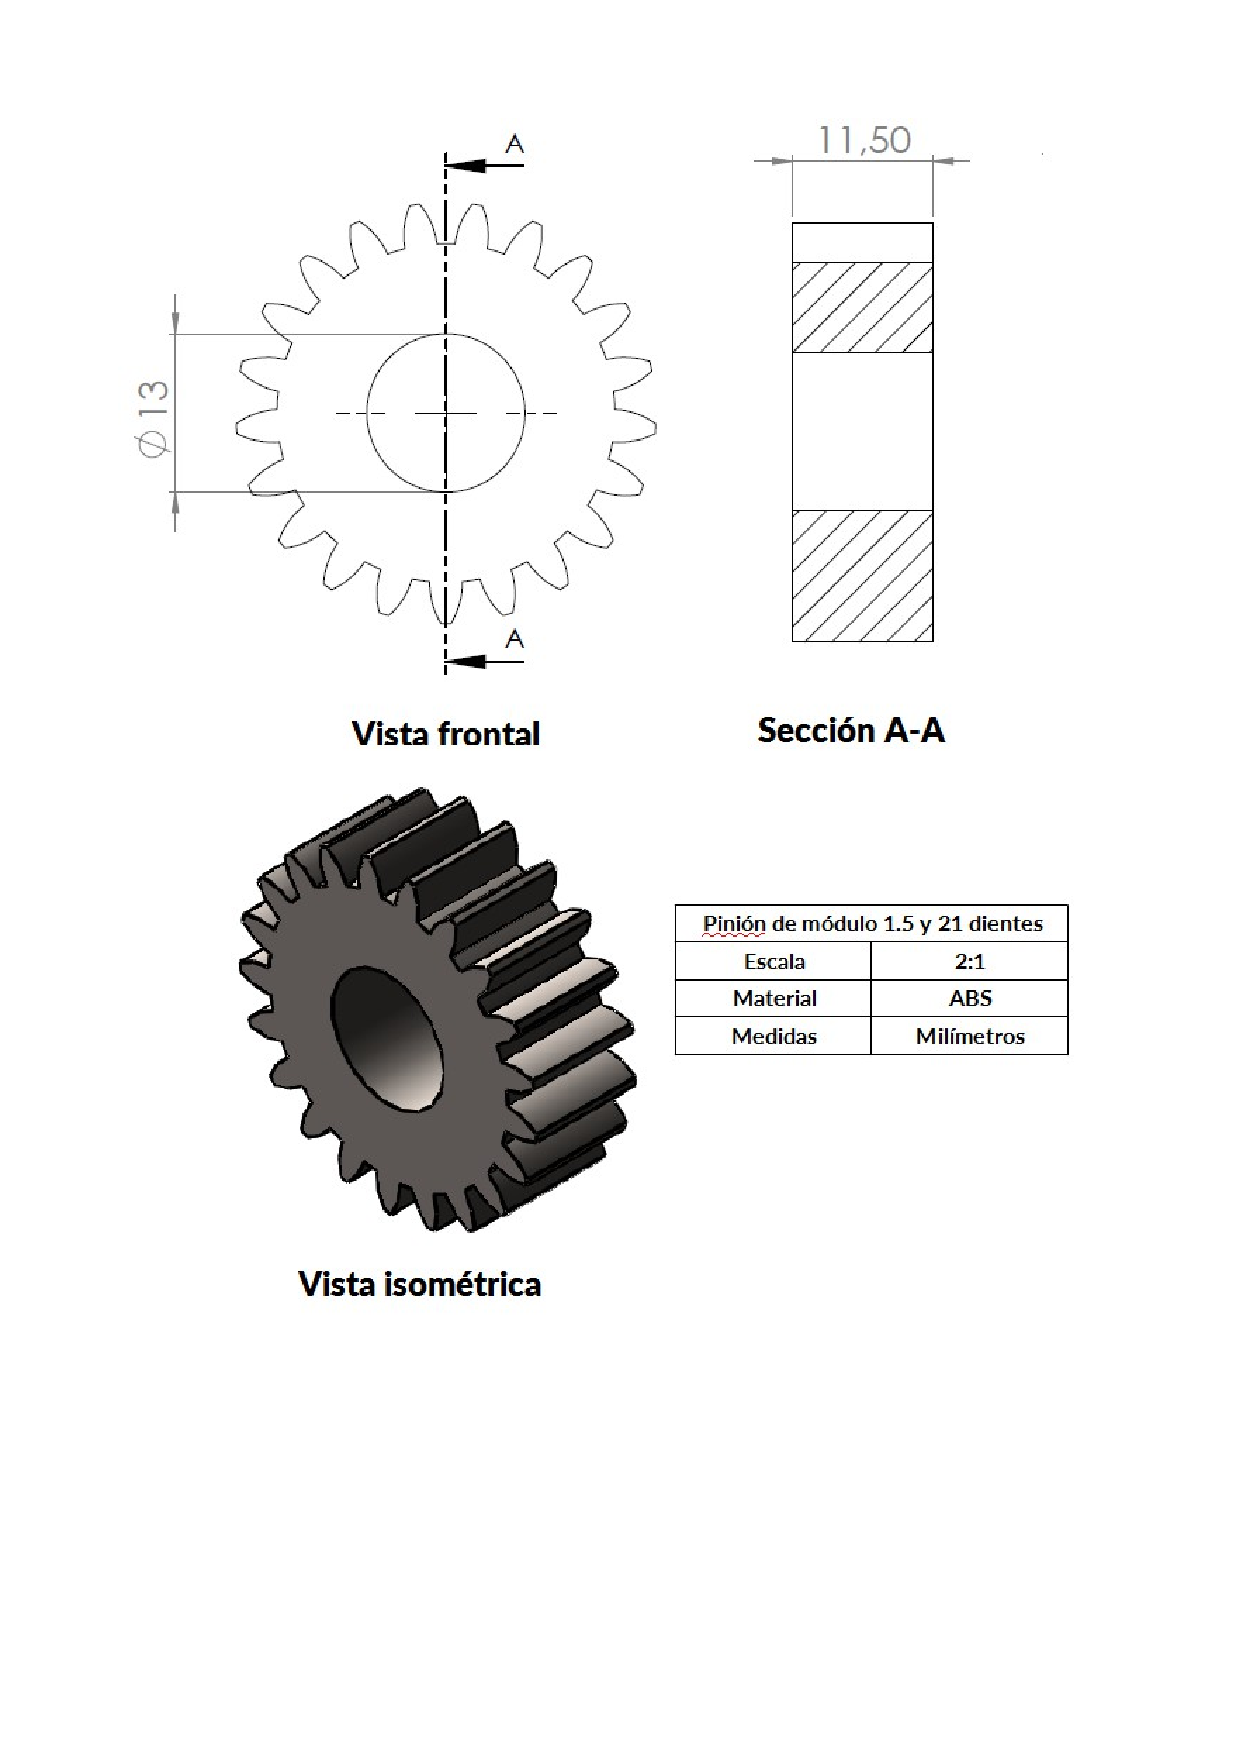
\includegraphics[width=\textwidth]{PlanoPinion.pdf}
\caption{Piñón.}
\end{figure}

\begin{figure}[ht]
\centering
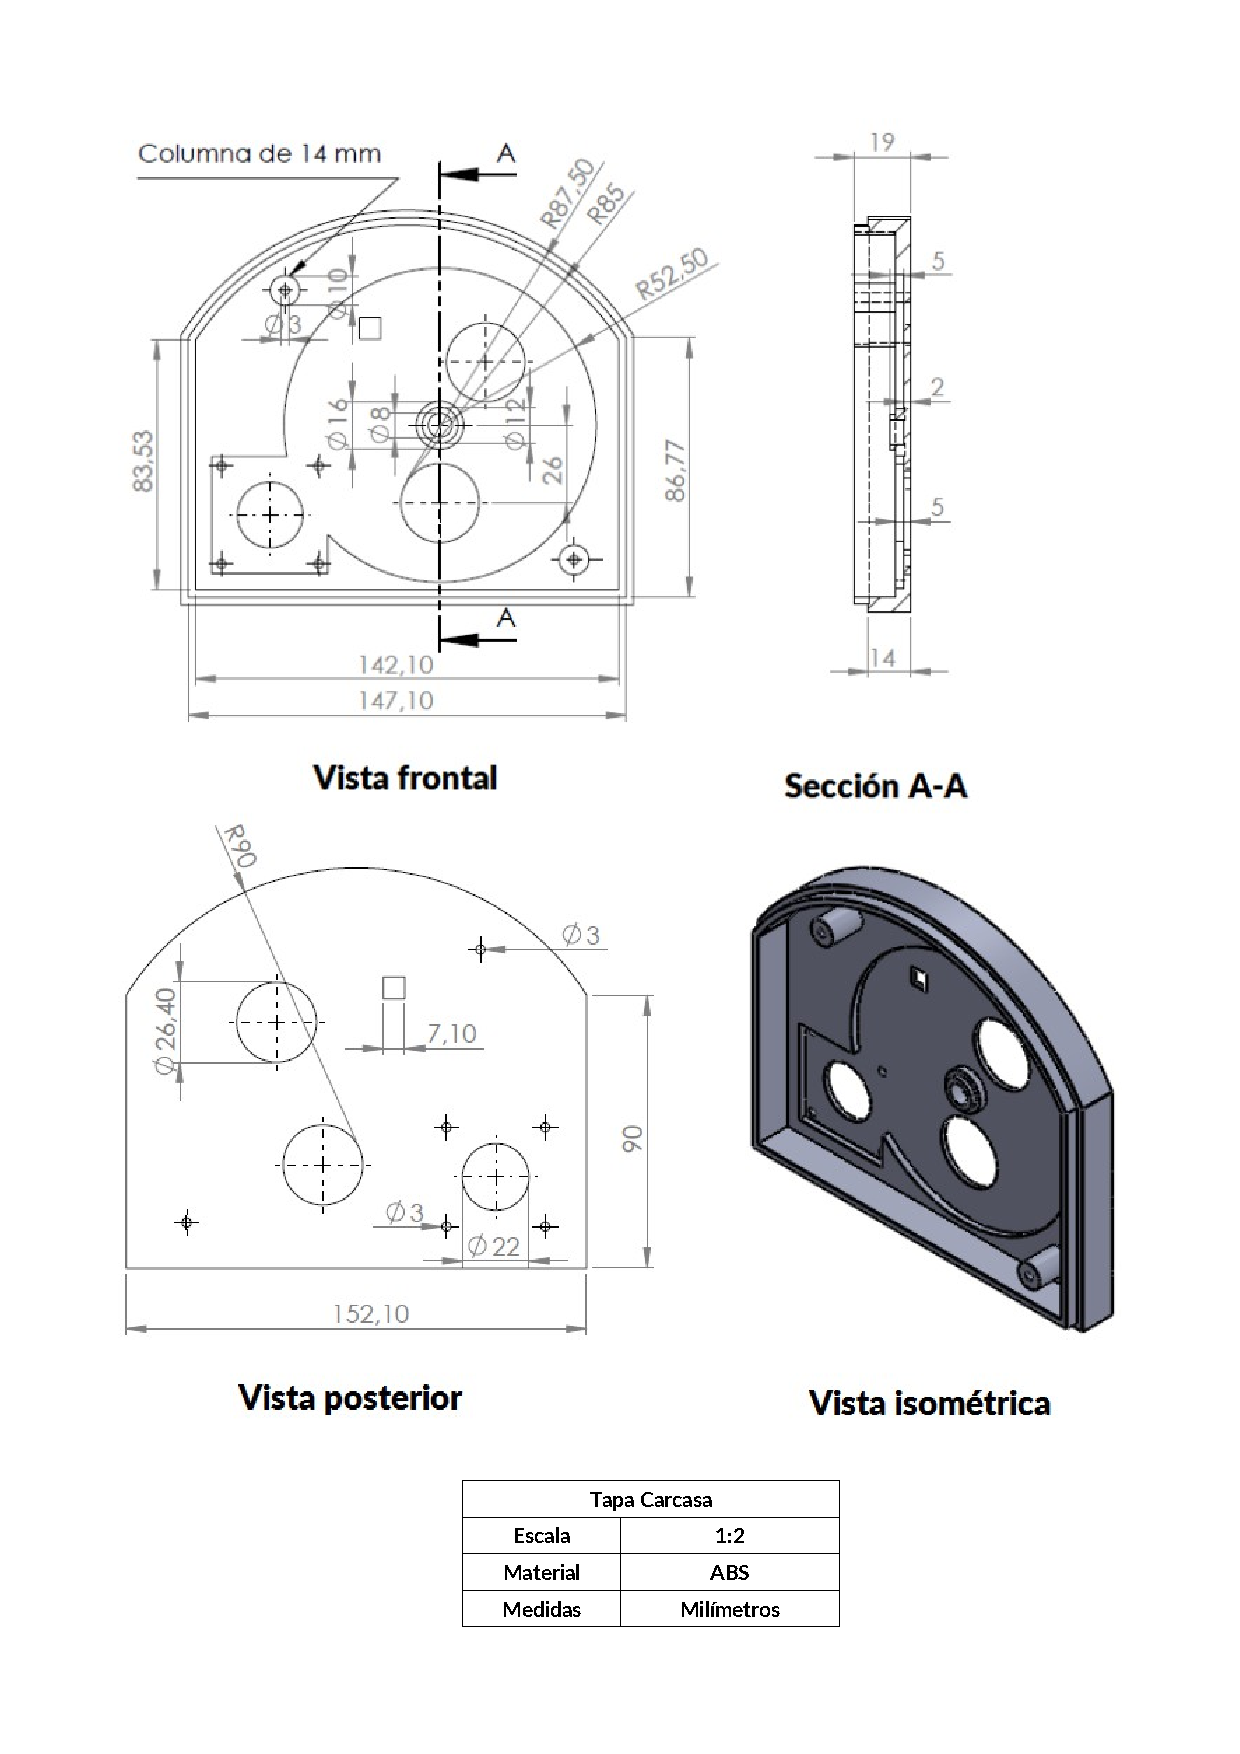
\includegraphics[width=\textwidth]{PlanoTapaCarcasa.pdf}
\caption{Piñón.}
\end{figure}

\begin{figure}[ht]
\centering
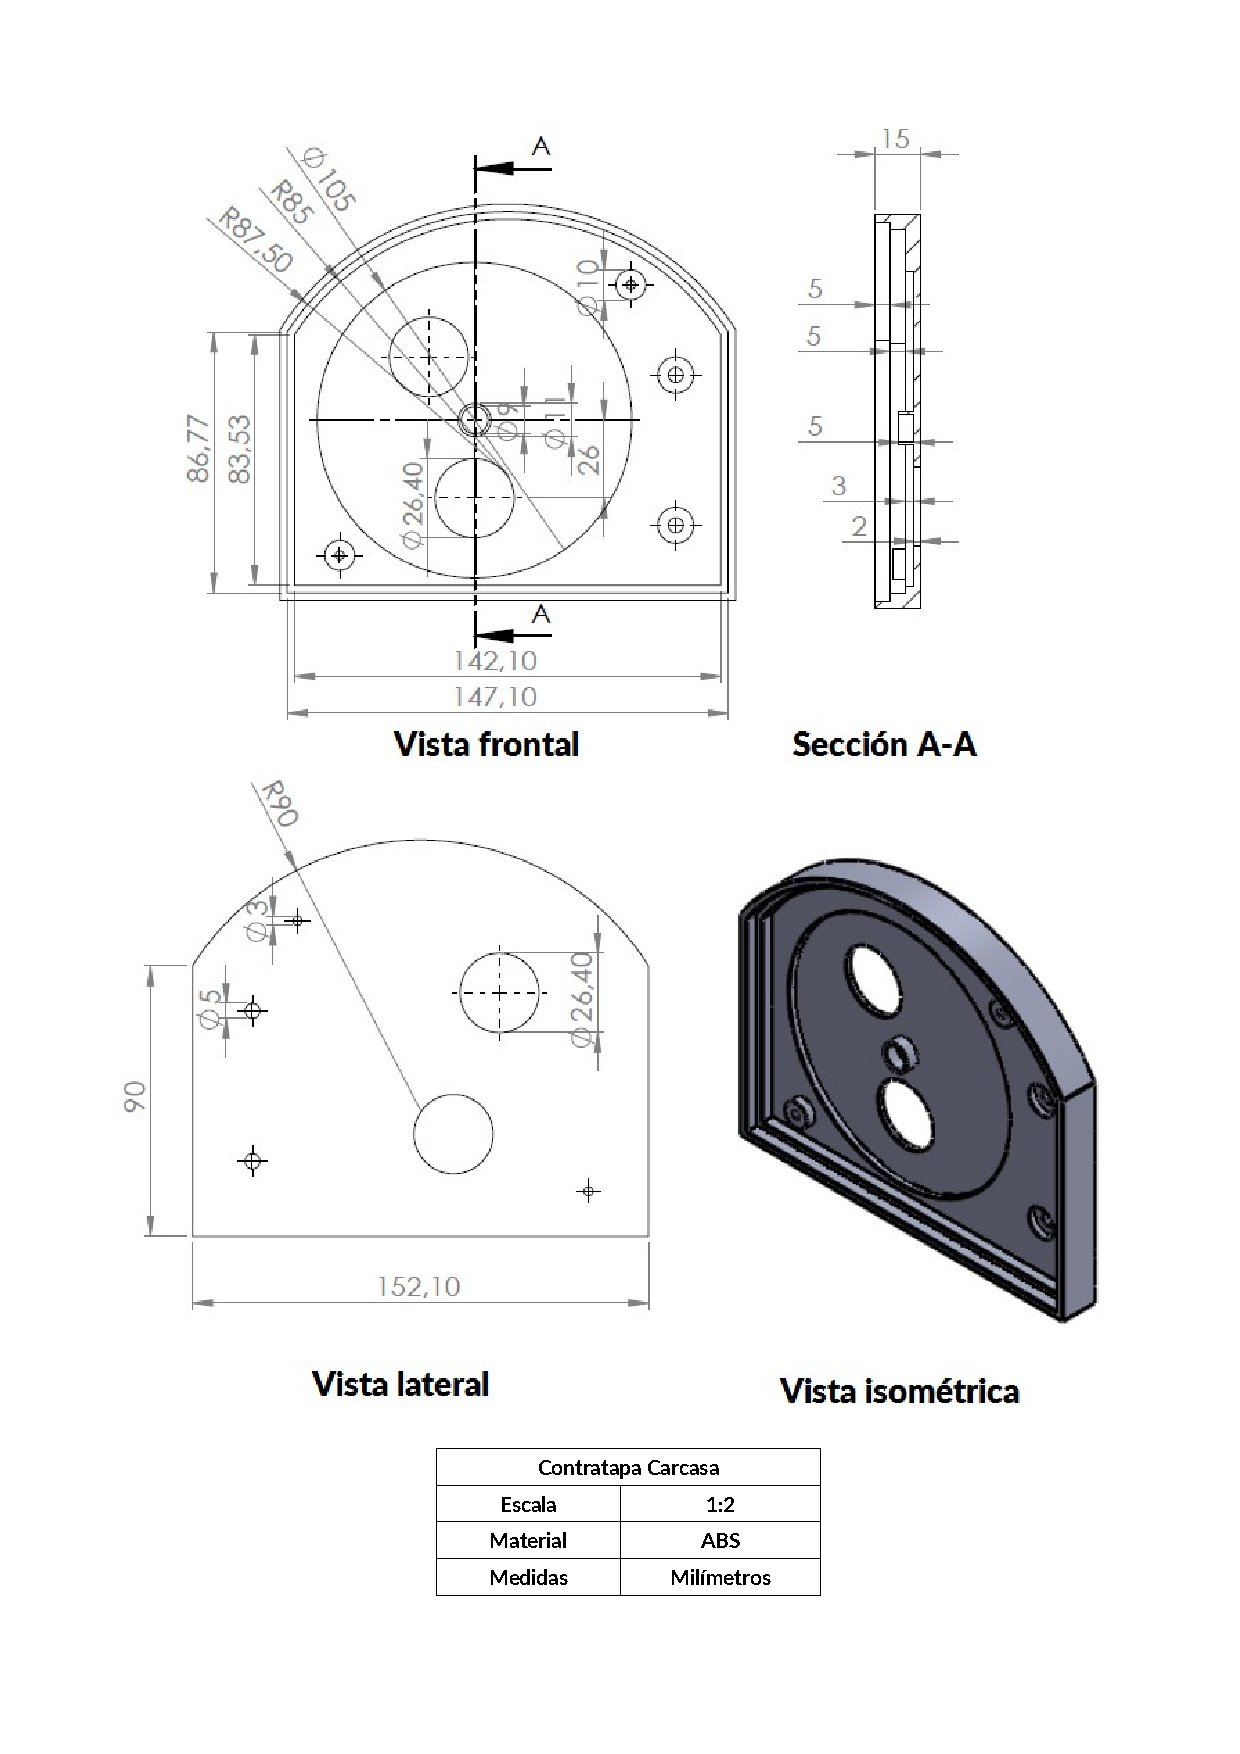
\includegraphics[width=\textwidth]{PlanoContratapaCarcasa.pdf}
\caption{Piñón.}
\end{figure}

\begin{figure}[ht]
\centering
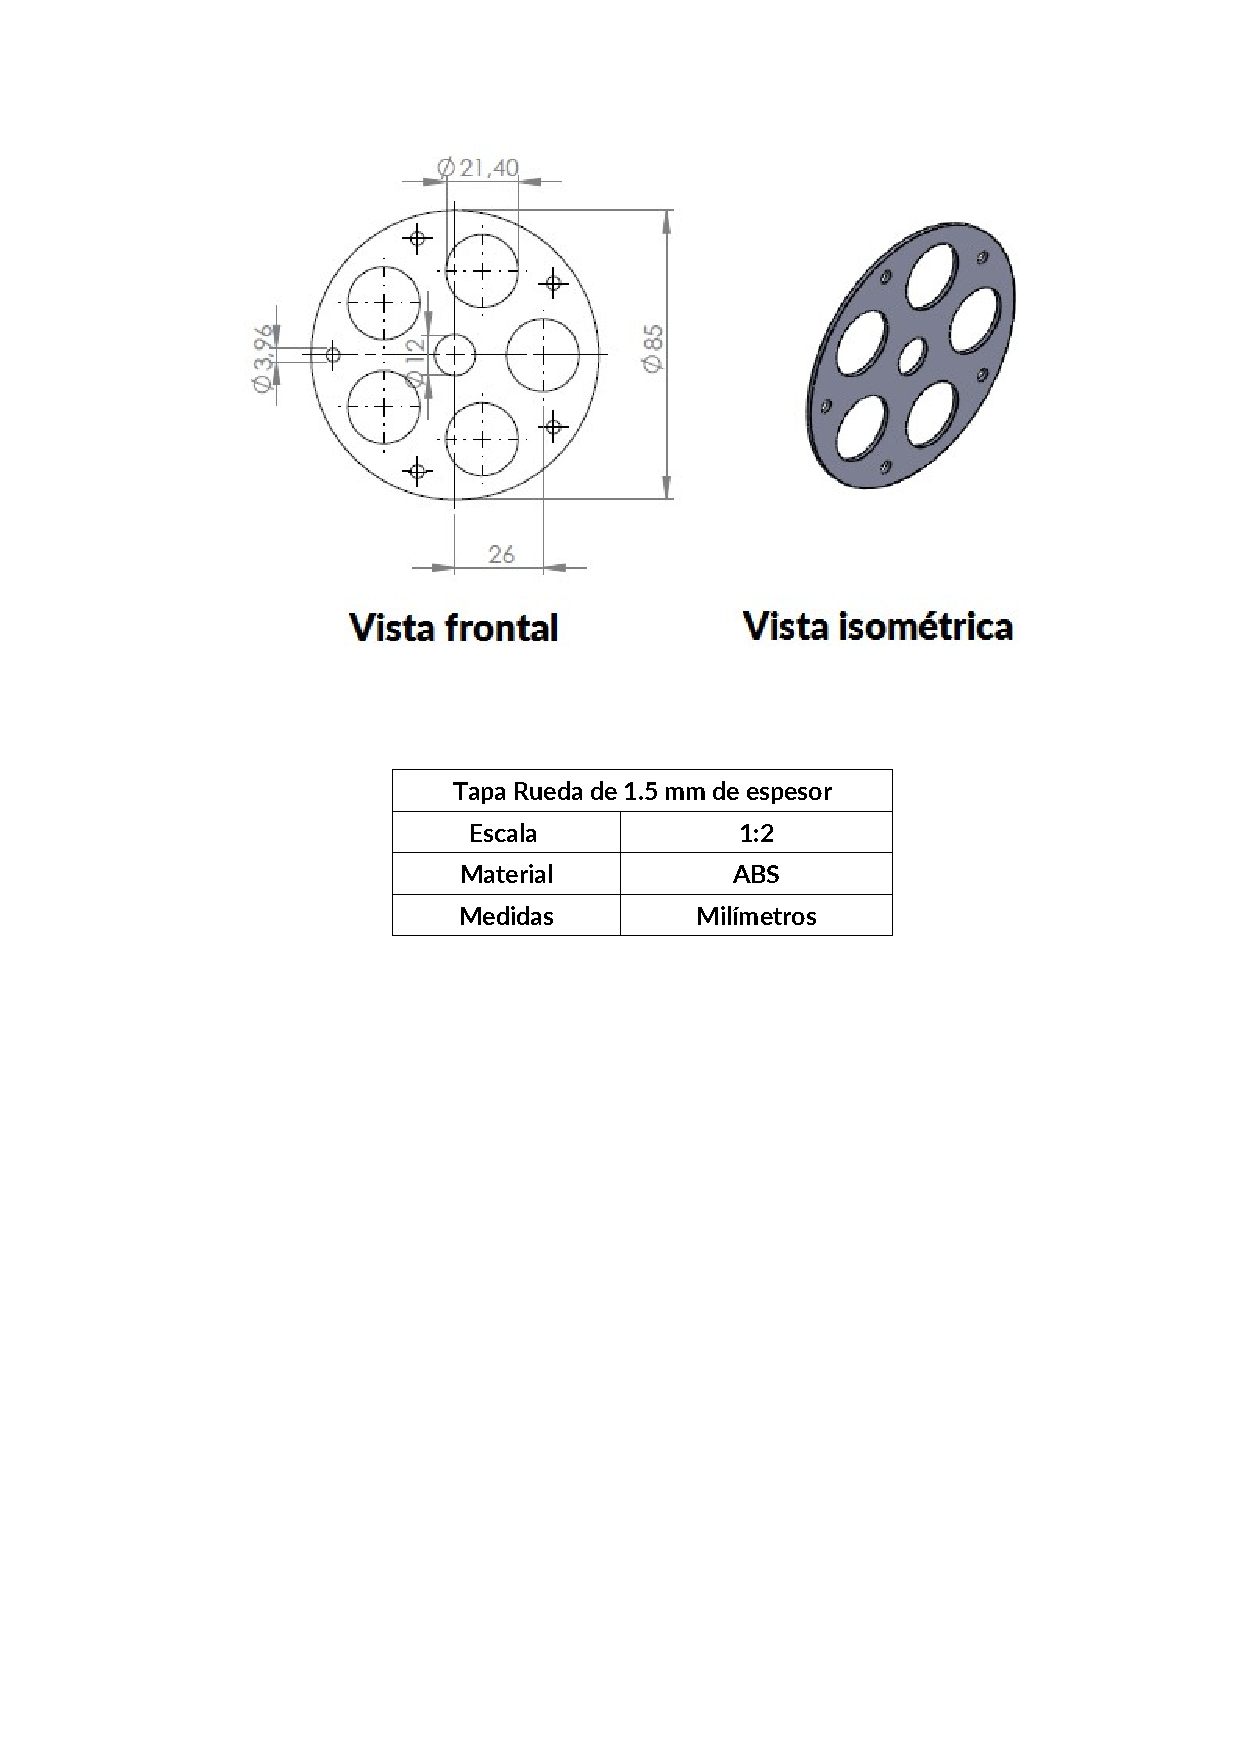
\includegraphics[width=\textwidth]{PlanoTapaRueda.pdf}
\caption{Piñón.}
\end{figure}

\end{document}